\documentclass[11pt,a4paper,twoside]{book}\usepackage[]{graphicx}\usepackage[]{color}
%% maxwidth is the original width if it is less than linewidth
%% otherwise use linewidth (to make sure the graphics do not exceed the margin)
\makeatletter
\def\maxwidth{ %
  \ifdim\Gin@nat@width>\linewidth
    \linewidth
  \else
    \Gin@nat@width
  \fi
}
\makeatother

\definecolor{fgcolor}{rgb}{0.345, 0.345, 0.345}
\newcommand{\hlnum}[1]{\textcolor[rgb]{0.686,0.059,0.569}{#1}}%
\newcommand{\hlstr}[1]{\textcolor[rgb]{0.192,0.494,0.8}{#1}}%
\newcommand{\hlcom}[1]{\textcolor[rgb]{0.678,0.584,0.686}{\textit{#1}}}%
\newcommand{\hlopt}[1]{\textcolor[rgb]{0,0,0}{#1}}%
\newcommand{\hlstd}[1]{\textcolor[rgb]{0.345,0.345,0.345}{#1}}%
\newcommand{\hlkwa}[1]{\textcolor[rgb]{0.161,0.373,0.58}{\textbf{#1}}}%
\newcommand{\hlkwb}[1]{\textcolor[rgb]{0.69,0.353,0.396}{#1}}%
\newcommand{\hlkwc}[1]{\textcolor[rgb]{0.333,0.667,0.333}{#1}}%
\newcommand{\hlkwd}[1]{\textcolor[rgb]{0.737,0.353,0.396}{\textbf{#1}}}%
\let\hlipl\hlkwb

\usepackage{framed}
\makeatletter
\newenvironment{kframe}{%
 \def\at@end@of@kframe{}%
 \ifinner\ifhmode%
  \def\at@end@of@kframe{\end{minipage}}%
  \begin{minipage}{\columnwidth}%
 \fi\fi%
 \def\FrameCommand##1{\hskip\@totalleftmargin \hskip-\fboxsep
 \colorbox{shadecolor}{##1}\hskip-\fboxsep
     % There is no \\@totalrightmargin, so:
     \hskip-\linewidth \hskip-\@totalleftmargin \hskip\columnwidth}%
 \MakeFramed {\advance\hsize-\width
   \@totalleftmargin\z@ \linewidth\hsize
   \@setminipage}}%
 {\par\unskip\endMakeFramed%
 \at@end@of@kframe}
\makeatother

\definecolor{shadecolor}{rgb}{.97, .97, .97}
\definecolor{messagecolor}{rgb}{0, 0, 0}
\definecolor{warningcolor}{rgb}{1, 0, 1}
\definecolor{errorcolor}{rgb}{1, 0, 0}
\newenvironment{knitrout}{}{} % an empty environment to be redefined in TeX

\usepackage{alltt}
% We load package by package and set package relevant parameters.
% Topics are summarized later
%%%%%%%%%%%%%%%%%%%%%%%%%%%%%%%%%%%%%%%%%%%%%%%%%%%%%%%%%%%%%%%%%%%%%%%%
% helping packages
\usepackage{ifthen}
\usepackage{calc}

\usepackage[T1]{fontenc}       % provides fonts having  accented characters 
\usepackage[latin1]{inputenc}  % allows the user to input accented characters directly from the keyboard

%%%%%%%%%%%%%%%%%%%%%%%%%%%%%%%%%%%%%%%%%%%%%%%%%%%%%%%%%%%%%%%%%%%%%%%%

\renewcommand{\baselinestretch}{1.2}
\renewcommand{\textfraction}{0}%0.2     % placement of figures
\renewcommand{\topfraction}{1}%.3
\renewcommand{\bottomfraction}{1}%.3
\renewcommand{\floatpagefraction}{1}%.3
\setcounter{bottomnumber}{3}%1

\textwidth6.3in
\textheight9.7in
\topmargin-45pt
\oddsidemargin-.15in
\evensidemargin.15in
\headsep30pt
\headheight15pt
%\footskip20pt


%%%%%%%%%%%%%%%%%%%%%%%%%%%%%%%%%%%%%%%%%%%%%%%%%%%%%%%%%%%%%%%%%%%%%%%%

\usepackage[dvipsnames]{xcolor}
\definecolor{fgcolor}{rgb}{0.345, 0.345, 0.345}
\definecolor{shadecolor}{rgb}{.97, .97, .97}
\definecolor{messagecolor}{rgb}{0, 0, 0}
\definecolor{warningcolor}{rgb}{1, 0, 1}
\definecolor{errorcolor}{rgb}{1, 0, 0}
\definecolor{DarkBlue}{rgb}{0,0,0.5451}
\definecolor{DarkGreen}{rgb}{0,0.39216,0}
\definecolor{LightYellow}{rgb}{1,1,.8}
\definecolor{orange}{rgb}{.9,0.3445,0}



%%%%%%%%%%%%%%%%%%%%%%%%%%%%%%%%%%%%%%%%%%%%%%%%%%%%%%%%%%%%%%%%%%%%%%%%
\usepackage{afterpage}
\usepackage{natbib}
\usepackage{upquote}

\usepackage[english]{babel}

%%%%%%%%%%%%%%%%%%%%%%%%%%%%%%%%%%%%%%%%%%%%%%%%%%%%%%%%%%%%%%%%%%%%%%%%%%%%%%%
%% maxwidth is the original width if it is less than linewidth
%% otherwise use linewidth (to make sure the graphics do not exceed the margin)
\makeatletter
\def\maxwidth{ %
  \ifdim\Gin@nat@width>\linewidth
    \linewidth
  \else
    \Gin@nat@width
  \fi
}
\makeatother

%%%%%%%%%%%%%%%%%%%%%%%%%%%%%%%%%%%%%%%%%%%%%%%%%%%%%%%%%%%%%%%%%%%%%%%%%%%%%%%%%%%%%%%%%%%%%%%%%%%%%%%%%%%%
% from fancyvrb
\usepackage{fancyhdr}
\usepackage{fancyvrb}
\DefineVerbatimEnvironment{Rcode}{Verbatim}{xleftmargin=2em,fontshape=sl,formatcom=\color{DarkGreen}}
\fvset{listparameters={\setlength{\topsep}{0pt}}}

%%%%%%%%%%%%%%%%%%%%%%%%%%%%%%%%%%%%%%%%%%%%%%%%%%%%%%%%%%%%%%%%%%%%%%%%%%%%%%%%%%%%%%%%%%%%%%%%%%%%%%%%%%%%%
\usepackage{float}
\usepackage{graphicx}
\usepackage[margin=2em,labelfont=bf]{caption}


%%%%%%%%%%%%%%%%%%%%%%%%%%%%%%%%%%%%%%%%%%%%%%%%%%%%%%%%%%%%%%%%%%%%%%%%
\usepackage[pdftex,plainpages=false,pdfpagelabels,pagebackref=true,colorlinks=true,pdfpagemode=UseOutlines]{hyperref}


%%%%%%%%
\usepackage{tabularx}
%%%%%%%%

%%%%%%%%%%%%%%%%%%%%%%%%%%%%%%%%%%%%%%%%%%%%%%%%%%%%%%%%%%%%%%%%%%%%%%%%
% now math stuff and other details...
\usepackage{amsmath,amsthm,amssymb}

\newtheorem{pro}{Property}[chapter]
\theoremstyle{definition}
\newtheorem{des}{Definition}[chapter]
\newtheorem{bsp}{Example}[chapter]
\newtheorem{rem}{Remark}[chapter]

\newcommand*\widebar[1]{%
  \vbox{%
    \hrule height 0.5pt%     % Line above with certain width
    \kern0.5ex%             % Distance between line and content
    \hbox{%
      \kern-0.1em%           % Distance between content and left side of box, negative values for lines shorter than content
      \ifmmode#1\else\ensuremath{#1}\fi%  % The content, typeset in dependence of mode
      \kern-0.1em%      % Distance between content and left side of box, negative values for lines shorter than content
    }% end of hbox
  }% end of vbox
}
\def\ds{\displaystyle}

\newcommand{\rr}[1]{{\ttfamily\slshape\color{DarkGreen} #1}}

\makeatletter


% clever trick to circumvent potential redefines after loading packages:
% \providecommand{\something}{}  % if it does not exist, it creates it.
%      has same syntax as \newcommand
% \renewcommand{\something}{....}
% TUGboat 29(2)


\makeatletter
%umdefinierung exisitierender befehle
\let\oldH\H
\let\oldL\L
\let\oldO\H
\let\oldS\S
\let\olda\a
\let\oldb\b
\let\oldc\c
\let\oldd\d
\let\oldk\k
\let\oldv\v
\let\oldl\l
\let\oldt\t
\let\oldu\u
\let\oldIJ\IJ
\let\oldP\P
\let\P\relax
\let\oldnorm\|

%\DefineVerbatimEnvironment{CodeInput}{Verbatim}{fontshape=sl}
%\DefineVerbatimEnvironment{CodeOutput}{Verbatim}{}

% some classical environments, up-right, with chapter numbering.
\theoremstyle{definition}
\newtheorem{definition}{Definition}[chapter]
\newtheorem{example}{Example}[chapter]
\newtheorem{remark}{Remark}[chapter]
\newtheorem{theorem}{Theorem}[chapter]



\renewcommand{\|}{|\!|}         % closer norm
\newcommand{\T}{{}^{\top}}
\newcommand\code[1]{{\tt#1}}



\newcounter{algo}
\newenvironment{algorithm}{%
  \begin{list}{
      (\arabic{algo})
    }{
      \usecounter{algo}
    }%
}{
  \end{list}
}

% some text abbreviation
\newcommand{\GLS}{\text{GLS}}
\newcommand{\RR}{\text{RR}}
\newcommand{\OR}{\text{OR}}
\newcommand{\WLS}{\text{WLS}}
\newcommand{\MLE}{\text{MLE}}
\newcommand{\OLS}{\text{OLS}}
\newcommand{\MAE}{\text{MAE}}
\newcommand{\MAD}{\text{MAD}}
\newcommand{\RMSE}{\text{RMSE}}
\newcommand{\SVAR}{\text{svar}} %silvanos new commands
\newcommand{\EVAR}{\text{evar}}
\newcommand{\LMG}{\text{LMG}}
\newcommand{\Rtwo}{\text{R}^2}



\newcommand{\ii}{\text{\i}}

\newcommand{\Bin}{\cB\mathit{\!i\!n}}
\newcommand{\Beta}{\cB\mathit{\!e\!t\!a}}
\newcommand{\Pois}{\cP\mathit{\!o\!i\!s\!s\!o\!n}}
\newcommand{\Exp}{\cE\mathit{\!x\!p}}


\DeclareMathOperator*{\argmin}{argmin}
\DeclareMathOperator*{\argmax}{argmax}
\DeclareMathOperator{\diag}{diag}
\DeclareMathOperator{\diam}{diam}
\DeclareMathOperator{\card}{card}
\DeclareMathOperator{\cov}{Cov}                   
\DeclareMathOperator{\corr}{Corr}                 
\DeclareMathOperator{\var}{Var}                   
\DeclareMathOperator{\trace}{tr}                  
\DeclareMathOperator{\E}{E}                       
\DeclareMathOperator{\P}{P}                       
\DeclareMathOperator{\pred}{p}
\DeclareMathOperator{\vect}{vec}                  
\DeclareMathOperator{\vech}{vech}                 
\DeclareMathOperator{\rank}{rank}                 
\DeclareMathOperator{\e}{e}                       
%\DeclareMathOperator{\cv}{CV}                     
\DeclareMathOperator{\GCV}{GCV}                     
\DeclareMathOperator{\CV}{CV}                     
\DeclareMathOperator{\BLUP}{BLUP}                 
\DeclareMathOperator{\MSE}{MSE}                   
\DeclareMathOperator{\MS}{MS}                   
\DeclareMathOperator{\df}{df}                   
\DeclareMathOperator{\bias}{bias}                   
\DeclareMathOperator{\eig}{eig}                   
\DeclareMathOperator{\Prec}{Prec}
\DeclareMathOperator{\mode}{mode}
\renewcommand{\SS}{\text{SS}}
\renewcommand{\d}{\mathsf{\,d}}

\def\arctanh{\qopname\relax o{arctanh}}  % as in amsopn
\newcommand{\bigo}{\cO}
\newcommand{\lito}{\text{\scriptsize{$\cO$}}}
\newcommand{\cdfPhi}{\itPhi}
\newcommand{\ml}{_\text{ML}}

\newcommand*{\stack@relbin}[3][]{%
  \mathop{#3}\limits
  \toks@{#1}%
  \edef\reserved@a{\the\toks@}%
  \ifx\reserved@a\@empty\else_{#1}\fi
  \toks@{#2}%
  \edef\reserved@a{\the\toks@}%
  \ifx\reserved@a\@empty\else^{#2}\fi
  \egroup
}%
\renewcommand*{\stackrel}{\mathrel\bgroup\stack@relbin}
\newcommand*{\stackbin}{\mathbin\bgroup\stack@relbin}
\newcommand{\simiid}{\stackrel[]{\text{iid}}{\sim}}

% Kalligraphischer Schriftsatz
\newcommand{\cA}{{\cal{A}}}
\newcommand{\cB}{{\cal{B}}} 
\newcommand{\cC}{{\cal{C}}}
\newcommand{\cD}{{\cal{D}}} 
\newcommand{\cE}{{\cal{E}}}
\newcommand{\cF}{{\cal{F}}}
\newcommand{\cG}{{\cal{G}}}
\newcommand{\cH}{{\cal{H}}}
\newcommand{\cI}{{\cal{I}}}
\newcommand{\cJ}{{\cal{J}}}
\newcommand{\cK}{{\cal{K}}}
\newcommand{\cL}{{\cal{L}}}
\newcommand{\cM}{{\cal{M}}} 
\newcommand{\cN}{{\cal{N}}}
\newcommand{\cO}{{\cal{O}}} 
\newcommand{\cP}{{\cal{P}}}
\newcommand{\cQ}{{\cal{Q}}} 
\newcommand{\cR}{{\cal{R}}} 
\newcommand{\cS}{{\cal{S}}} 
\newcommand{\cT}{{\cal{T}}}
\newcommand{\cU}{{\cal{U}}}
\newcommand{\cV}{{\cal{V}}}
\newcommand{\cW}{{\cal{W}}}
\newcommand{\cX}{{\cal{X}}} 
\newcommand{\cY}{{\cal{Y}}}
\newcommand{\cZ}{{\cal{Z}}} 


\newcommand{\IA}{{\mathbb{A}}}
\newcommand{\IB}{{\mathbb{B}}}
\newcommand{\IC}{{\mathbb{C}}}
\newcommand{\ID}{{\mathbb{D}}}
\newcommand{\IE}{{\mathbb{E}}}
\newcommand{\IF}{{\mathbb{F}}}
\newcommand{\IG}{{\mathbb{G}}}
\newcommand{\IH}{{\mathbb{H}}}
\newcommand{\II}{{\mathbb{I}}}
%\newcommand{\IJ}{{\mathbb{J}}}
\newcommand{\IK}{{\mathbb{K}}}
\newcommand{\IL}{{\mathbb{L}}}
\newcommand{\IM}{{\mathbb{M}}}
\newcommand{\IN}{{\mathbb{N}}}
\newcommand{\IO}{{\mathbb{O}}}
\newcommand{\IP}{{\mathbb{P}}}
\newcommand{\IQ}{{\mathbb{Q}}}
\newcommand{\IR}{{\mathbb{R}}}
\newcommand{\IS}{{\mathbb{S}}}
\newcommand{\IT}{{\mathbb{T}}}
\newcommand{\IU}{{\mathbb{U}}}
\newcommand{\IV}{{\mathbb{V}}}
\newcommand{\IW}{{\mathbb{W}}}
\newcommand{\IX}{{\mathbb{X}}}
\newcommand{\IY}{{\mathbb{Y}}}
\newcommand{\IZ}{{\mathbb{Z}}}


% fette griechische kleinbuchstaben
\newcommand{\balpha}{{\boldsymbol{\alpha}}}
\newcommand{\bbeta}{{\boldsymbol{\beta}}}
\newcommand{\bgamma}{{\boldsymbol{\gamma}}}
\newcommand{\bdelta}{{\boldsymbol{\delta}}}
\newcommand{\blambda}{{\boldsymbol{\lambda}}}
\newcommand{\bepsilon}{{\boldsymbol{\epsilon}}}
\newcommand{\bvarepsilon}{{\boldsymbol{\varepsilon}}}
\newcommand{\bzeta}{{\boldsymbol{\zeta}}}
\newcommand{\bfeta}{{\boldsymbol{\eta}}}  %  <----- exception !
\newcommand{\btheta}{{\boldsymbol{\theta}}{}}
\newcommand{\bvartheta}{{\boldsymbol{\vartheta}}}
\newcommand{\biota}{{\boldsymbol{\iota}}}
\newcommand{\bkappa}{{\boldsymbol{\kappa}}}
\newcommand{\bmu}{{\boldsymbol{\mu}}}
\newcommand{\bnu}{{\boldsymbol{\nu}}}
\newcommand{\bxi}{{\boldsymbol{\xi}}}
\newcommand{\bpi}{{\boldsymbol{\pi}}}
\newcommand{\bvarpi}{{\boldsymbol{\varpi}}}
\newcommand{\brho}{{\boldsymbol{\rho}}}
\newcommand{\bvarrhoi}{{\boldsymbol{\varrho}}}
\newcommand{\bsigma}{{\boldsymbol{\sigma}}}
\newcommand{\bvarsigma}{{\boldsymbol{\varsigma}}}
\newcommand{\btau}{{\boldsymbol{\tau}}}
\newcommand{\bvartau}{{\boldsymbol{\vartau}}}
\newcommand{\bupsilon}{{\boldsymbol{\upsilon}}}
\newcommand{\bphi}{{\boldsymbol{\phi}}}
\newcommand{\bvarphi}{{\boldsymbol{\varphi}}}
\newcommand{\bchi}{{\boldsymbol{\chi}}}
\newcommand{\bpsi}{{\boldsymbol{\psi}}}
\newcommand{\bomega}{{\boldsymbol{\omega}}}


% fette griechische grossbuchstaben
\newcommand{\bGamma}{{\boldsymbol{\Gamma}}}
\newcommand{\bDelta}{{\boldsymbol{\Delta}}}
\newcommand{\bTheta}{{\boldsymbol{\Theta}}}
\newcommand{\bLambda}{{\boldsymbol{\Lambda}}{}}
\newcommand{\bXi}{{\boldsymbol{\Xi}}}
\newcommand{\bPi}{{\boldsymbol{\Pi}}}
\newcommand{\bSigma}{{\boldsymbol{\Sigma}}{}}
\newcommand{\bUpsilon}{{\boldsymbol{\Upsilon}}{}}
\newcommand{\bPhi}{{\boldsymbol{\Phi}}}
\newcommand{\bPsi}{{\boldsymbol{\Psi}}}
\newcommand{\bOmega}{{\boldsymbol{\Omega}}}

% italics griechische grossbuchstaben
\newcommand{\itGamma}{{\mathit{\Gamma}}}
\newcommand{\itDelta}{{\mathit{\Delta}}}
\newcommand{\itTheta}{{\mathit{\Theta}}}
\newcommand{\itLambda}{{\mathit{\Lambda}}}
\newcommand{\itXi}{{\mathit{\Xi}}}
\newcommand{\itPi}{{\mathit{\Pi}}}
\newcommand{\itSigma}{{\mathit{\Sigma}}}
\newcommand{\itUpsilon}{{\mathit{\Upsilon}}}
\newcommand{\itPhi}{{\mathit{\Phi}}}
\newcommand{\itPsi}{{\mathit{\Psi}}}
\newcommand{\itOmega}{{\mathit{\Omega}}}



\newcommand{\A}{{\mathbf{A}}}
\newcommand{\B}{{\mathbf{B}}}
\newcommand{\C}{{\mathbf{C}}}
\newcommand{\D}{{\mathbf{D}}}
\newcommand{\bfE}{{\mathbf{E}}}    % \E: expectation
\newcommand{\F}{{\mathbf{F}}}
\newcommand{\G}{{\mathbf{G}}}
\renewcommand{\H}{{\mathbf{H}}}
\newcommand{\I}{{\mathbf{I}}}
\newcommand{\J}{{\mathbf{J}}}
\newcommand{\K}{{\mathbf{K}}}
\renewcommand{\L}{{\mathbf{L}}}
\newcommand{\bfM}{{\mathbf{M}}}
\newcommand{\N}{{\mathbf{N}}}
\renewcommand{\O}{{\mathbf{O}}}
\newcommand{\bfP}{{\mathbf{P}}}  % \P : probability
\newcommand{\Q}{{\mathbf{Q}}}
\newcommand{\bfR}{{\mathbf{R}}}
\renewcommand{\S}{{\mathbf{S}}}
\newcommand{\bfT}{{\mathbf{T}}} % \T transpose
\newcommand{\U}{{\mathbf{U}}}
\newcommand{\V}{{\mathbf{V}}}
\newcommand{\W}{{\mathbf{W}}}
\newcommand{\X}{{\mathbf{X}}}
\newcommand{\Y}{{\mathbf{Y}}}
\newcommand{\Z}{{\mathbf{Z}}}


\newcommand{\0}{{\mathbf{0}}}
\newcommand{\1}{{\mathbf{1}}}
\newcommand{\2}{{\mathbf{2}}}
\newcommand{\3}{{\mathbf{3}}}
\newcommand{\4}{{\mathbf{4}}}
\newcommand{\5}{{\mathbf{5}}}
\newcommand{\6}{{\mathbf{6}}}
\newcommand{\7}{{\mathbf{7}}}
\newcommand{\8}{{\mathbf{8}}}
\newcommand{\9}{{\mathbf{9}}}

\renewcommand{\a}{{\textbf{\textit{a}}}}
\renewcommand{\b}{{\textbf{\textit{b}}}}
\renewcommand{\c}{{\textbf{\textit{c}}}}
\newcommand{\bfd}{{\textbf{\textit{d}}}}  % \d  'dx'
\newcommand{\bfe}{{\textbf{\textit{e}}}}  % \e  l'exponentiel
\newcommand{\f}{{\textbf{\textit{f}}}}
\newcommand{\g}{{\textbf{\textit{g}}}}
\newcommand{\h}{{\textbf{\textit{h}}}}
\newcommand{\bfi}{{\textbf{\textit{i}}}}%\i  complex i, sans 'dot'
\newcommand{\bfj}{{\textbf{\textit{j}}}}
\renewcommand{\l}{{\textbf{\textit{l}}}}
\renewcommand{\k}{{\textbf{\textit{k}}}}
\newcommand{\m}{{\textbf{\textit{m}}}}
\newcommand{\bfn}{{\textbf{\textit{n}}}}
\newcommand{\bfo}{{\textbf{\textit{o}}}}
\newcommand{\p}{{\textbf{\textit{p}}}}
\newcommand{\q}{{\textbf{\textit{q}}}}
\renewcommand{\r}{{\textbf{\textit{r}}}}
\newcommand{\s}{{\textbf{\textit{s}}}}
\renewcommand{\t}{{\textbf{\textit{t}}}}
\newcommand{\bfu}{{\textbf{\textit{u}}}} %\u used in references
\renewcommand{\v}{{\textbf{\textit{v}}}}
\newcommand{\w}{{\textbf{\textit{w}}}}
\newcommand{\x}{{\textbf{\textit{x}}}}
\newcommand{\y}{{\textbf{\textit{y}}}}
\newcommand{\z}{{\textbf{\textit{z}}}}




\ifcsname hlkwd\endcsname%    ... command '#1' exists ...%
\else%  ... command '#1' does not exist ...%

\def\maxwidth{ %
  \ifdim\Gin@nat@width>\linewidth
    \linewidth
  \else
    \Gin@nat@width
  \fi
}

\definecolor{fgcolor}{rgb}{0.345, 0.345, 0.345}
\newcommand{\hlnum}[1]{\textcolor[rgb]{0.686,0.059,0.569}{#1}}%
\newcommand{\hlstr}[1]{\textcolor[rgb]{0.192,0.494,0.8}{#1}}%
\newcommand{\hlcom}[1]{\textcolor[rgb]{0.678,0.584,0.686}{\textit{#1}}}%
\newcommand{\hlopt}[1]{\textcolor[rgb]{0,0,0}{#1}}%
\newcommand{\hlstd}[1]{\textcolor[rgb]{0.345,0.345,0.345}{#1}}%
\newcommand{\hlkwa}[1]{\textcolor[rgb]{0.161,0.373,0.58}{\textbf{#1}}}%
\newcommand{\hlkwb}[1]{\textcolor[rgb]{0.69,0.353,0.396}{#1}}%
\newcommand{\hlkwc}[1]{\textcolor[rgb]{0.333,0.667,0.333}{#1}}%
\newcommand{\hlkwd}[1]{\textcolor[rgb]{0.737,0.353,0.396}{\textbf{#1}}}%

\usepackage{framed}
\newenvironment{kframe}{%
 \def\at@end@of@kframe{}%
 \ifinner\ifhmode%
  \def\at@end@of@kframe{\end{minipage}}%
  \begin{minipage}{\columnwidth}%
 \fi\fi%
 \def\FrameCommand##1{\hskip\@totalleftmargin \hskip-\fboxsep
 \colorbox{shadecolor}{##1}\hskip-\fboxsep
     % There is no \\@totalrightmargin, so:
     \hskip-\linewidth \hskip-\@totalleftmargin \hskip\columnwidth}%
 \MakeFramed {\advance\hsize-\width
   \@totalleftmargin\z@ \linewidth\hsize
   \@setminipage}}%
 {\par\unskip\endMakeFramed%
 \at@end@of@kframe}
\renewenvironment{kframe}{%
 \def\at@end@of@kframe{}%
 \ifinner\ifhmode%
  \def\at@end@of@kframe{\end{minipage}}%
  \begin{minipage}{\columnwidth}%
 \fi\fi%
 \def\FrameCommand##1{\hskip\@totalleftmargin \hskip-0\fboxsep
 \colorbox{shadecolor}{##1}\hskip-0\fboxsep
     % There is no \\@totalrightmargin, so:
     \hskip-\linewidth \hskip-\@totalleftmargin \hskip\columnwidth}%
 \MakeFramed {\advance\hsize-\width
   \@totalleftmargin\z@ \linewidth\hsize
   \@setminipage}}%
 {\par\unskip\endMakeFramed%
 \at@end@of@kframe}


\definecolor{shadecolor}{rgb}{.97, .97, .97}
\definecolor{messagecolor}{rgb}{0, 0, 0}
\definecolor{warningcolor}{rgb}{1, 0, 1}
\definecolor{errorcolor}{rgb}{1, 0, 0}
%\newenvironment{knitrout}{}{} % an empty environment to be redefined in TeX
\newenvironment{knitrout}{\setlength{\topsep}{0mm}\setlength{\fboxsep}{4mm}}{} 

\usepackage{alltt}
\IfFileExists{upquote.sty}{\usepackage{upquote}}{}

  \fi%

\makeatother
   % packages, layout and standard macros
\IfFileExists{upquote.sty}{\usepackage{upquote}}{}
\begin{document}
\renewcommand\familydefault{\sfdefault} 
\pagenumbering{Alph}


\thispagestyle{empty}
\renewcommand{\baselinestretch}{1.5}\normalfont
\begin{center}
\setlength{\parindent}{0cm}
\bf\Large% 
The variable importance metric LMG  \\
applied to Bayesian linear regression models
\normalfont



\hrulefill

\vspace*{4cm}

\large
Master Thesis in Biostatistics (STA495) % or choose the next one
% Master Thesis in Mathematics (MAT491) 
\vspace*{12mm}

by

\vspace*{12mm}

Silvano Sele\\
\small 09 734 492\\
\normalfont
\vspace*{4cm}

supervised by

\vspace*{1cm}

Dr. Stefanie Muff\\
Name of supervisor (with title and affiliation if external)

\vfill

Zurich, September, 2018
\end{center}
\renewcommand\familydefault{\rmdefault}%
\renewcommand{\baselinestretch}{1.0}\rm 
\setcounter{page}{0}
\newpage
\vspace*{12cm}~\thispagestyle{empty}\pagenumbering{Roman}
\newpage


\graphicspath{{./figure/}}
\DeclareGraphicsExtensions{.pdf,.png}
\setcounter{tocdepth}{1}

\thispagestyle{empty}
\begin{center}
\vspace*{6cm}{\bfseries\Huge
  $p$-values:\\[5mm] their use, abuse and proper use \\[5mm]
  illustrated with seven facets 
}
\vfill
\rm

\LARGE
M\"axli Musterli\\[12mm]

\normalsize
Version \today
\end{center}
\newpage
\thispagestyle{empty}~
\newpage
\pagenumbering{roman}

\thispagestyle{plain}\markboth{Contents}{Contents}
\tableofcontents
\setkeys{Gin}{width=.8\textwidth}

\chapter*{Preface}
\addtocontents{toc}{\protect \vspace*{13.mm}}
\addcontentsline{toc}{chapter}{\bfseries{Preface}}
\thispagestyle{plain}\markboth{Preface}{Preface}

Howdy!

\bigskip

\begin{flushright}
Max Muster\\
June 2018
\end{flushright}

\addtocontents{toc}{\protect \vspace*{10mm}}

\cleardoublepage
\pagenumbering{arabic}


%%%%%%%%%%%%%%%%%%%%%%%%%%%%%%%%%%%%%%%%%%%%%%%%%%%%%%%%%%%%%%%%%%%%%% 



% LaTeX file for Chapter 01







\chapter{Introduction}

The aim of this master thesis is to implement the variable importance measure LMG (named after the authors Lindeman, Merenda, and Gold ref groemping 2007) in linear models estimated with Bayesian methods. 

Regression models are popular in many applied research areas. These models provide a tool to find an association between a response variable Y and a set of explanatory variables. These explanatory variables are also called predictors or covariates. Regression parameters provide us the information how much the response variable is expected to change when a predictor changes by one unit, given all other predictors in the model stay the same. The last subsentence is very important for the correct interpretation of the regression parameters. It shows also that the parameter value of a predictor is dependent on the other predictors in the model. Because predictors are often correlated to some degree to each other, it is clear that it is not an easy task to find the most important predictors in a model. The first question then is: What do we  mean by the importance of a predictor? A question that is not easy answered and depending on the research question. Goering 2015 concludes that there may never  be a unique accepted definition of what variable importance is.   Different metrics exist to quantify the importance of predictors. These metrics focus on different aspects and with correlated predictors they  lead to different conclusions. A distinction should be made between the importance of predictors in regression models that are used to predict future data and regression models who wish to find an association between predictors and the response variable. In the former case, the aim is only to reduce the error between the predicted values and the real observed values. It does not really matter how we get there. In the other case, we are interested in the strength of the relationship between the predictors and the response variable. A predictor may explain little of the response variable given two other correlated predictors are already included in a regression model. However, this from the regression output unimportant predictor may be the main cause of the other two predictor values.  It therefore may somehow be the most important predictor in this model. The causal relationship between the variables is missing in the regression model. Regressing conditional on  other variables or using univariate regression models only provide us some parts of the bigger picture about the predictor in a model. Some authors recommend that the variable importance metric is based on both components. Which variable importance metrics are the most useful ones is still an open debate. A convincing theoretical basis is still lacking for all of them. A summary of the metrics can be found in ref (groemping, 2015). Groemping 2015 recommends to use the existing best practices, until a more profound solution is found. For variance (or genereally goodness of fit) decomposition based importance she recommend to use LMG enhanced with joint contributions or dominance analysis.  

The focus of this master thesis is on the LMG variable importance metric. The LMG is a metric that is based on variance decomposition. The total $\Rtwo$ of a model is decomposed onto the predictors. Many authors call this a desirable property of a variable importance metric. Marginal and conditional information are incorporated.  The following formulas are taken from Groemping 2015. The same mathematical notations are used. 

The following  notations for the explained variance (1) and sequentially added variance (2) simplify the notation of the LMG formula. 

   \begin{align} 
     \EVAR(S) = \var(Y) - \var( Y \mid X_{j}, j \in S),   \label{eq:1} 
   \end{align} 
   \begin{align} 
     \SVAR(M \mid S) = \EVAR(M \cup S) - \EVAR(S), \label{eq:2} 
    \end{align} , where S and M denote disjoint sets of predictors.
    
 $\Rtwo(S)$ can be written as $\EVAR(S)/\var(Y).$   
   
  The LMG formula is given below for the first predictor only. Because of exchangeable predictors, this is no loss of generality.

   \begin{align} 
     \LMG(1) &= \frac{1}{p!} \sum_{\pi permutation}^{} \SVAR(\{1\} \mid S_{1}(\pi)),   \nonumber  \\
     &= \frac{1}{p!} \sum_{S \subseteq \{ 2, \dots, p \} }^{} n(S)!(p-n(S)-1)! \SVAR(\{1\} \mid S) \nonumber  \\
     &=  \cfrac{1}{p} \sum_{i=0}^{p-1} \left( \substack {\sum\limits_{ S \subseteq \{ 2, \dots, p \}}\\n(S)=1}^{} \ \SVAR(\{1\} \mid S)\right)\bigg/ \binom{p-1}{i}\\   
         &=  \cfrac{1}{p} \sum_{i=0}^{p-1} \frac{ \substack{\sum\limits_{ S \subseteq \{ 2, \dots, p \}}\\n(S)=1}^{} \ \SVAR(\{1\} \mid S)}{\binom{p-1}{i}} \\      
   \end{align},
   where $S_{1}(\pi)$ is the set of predecessors of predictor 1.
   
   The different writings of the formulas help to better grasp what is calculated in the LMG metric. The $\Rtwo$ of the model including all predictors is decomposed. In the top formula the LMG value of predictor 1 is represented as an unweighted average over all orderings of the sequentiel added variance contribution of predictor 1. The middle formula shows that the calculation can be  done computationally more efficient. The orderings with the same set of predecessors $S$ are combined into one summand. Instead of $p!$ summands only $2^{p-1}$ summands need to be calculated. The bottom formula shows that the LMG metric can also be seen as the unweighted average over average explained variance improvements when adding predictor 1 to a model of size i without predictor 1. 
   
The LMG metric is implemented in the R packages relaimpo and hier.part.

Chevan and Sutherland propose that instead of the variances an appropriate goodness-of-fit metric can be used in the LMG formula. They name their proposal hierarchical partitioning. The requirements are simply: an initial measure of fit when no predictor variable is present, a final measure of fit when N predictor variables are present, all intermediate models when various combinations of predictor variables are present. 
Hierarchical partitioning is implemented in the hier.part package. The LMG component of each variable is named independent component (I). The sum of the independent components (I) results then in the overall goodness-of-fit metric. The difference between the goodness-of-fit when only the predictors itself is included in the model, compared to its independent component (I) is named the joint contribution (J).  

For the linear model the $\Rtwo$ is the most widely used goodness-of-fit metric. Different formulas for $\Rtwo$ exist (Kvalseth, 1985), all leading to the same value when and intercept is included and the model is fitted by maximum likelihood. 

Two popular definitions are:
   
      \begin{align} 
     R^2 &= 1 - \frac{\sum_{i=1}^{n}(y_{i} - \hat{y_{i}})^2}{\sum_{i=1}^{n}(y_{i}-\bar{y})^2}   \label{eq:4}  \\
     R^2 &= \frac{\sum_{i=1}^{n}(\hat{y_{i}} - \bar{y})^2}{\sum_{i=1}^{n}(y_{i}-\bar{y})^2}   \label{eq:5} 
   \end{align} 
   
, where $\hat{y_{i}} = = \E ({y \mid X_{n}, \hat{\theta}})$.  

When other estimation methods than maximum likelihood are used (4) can be negative and (5) can be bigger than 1. When the model is fitted by Baysian methods and estimates of the posteriors are employed this can easily happen (Gelman). A model that explaines more than 100\% of the variance does not make sense. A negative $\Rtwo$ is also difficult to interpret. A negative $\Rtwo$ may be interpreted as a fit that is worse than the mean of the data. When new data from a test set is predicted (e.g. in leave-one-out crossvalidation), one has to be careful with the $\Rtwo$ definition used. $R^2$ should then be calculated by equation(4). Negative $R^2$ can then also happen, when the model is fitted by maximum likelihood (Referenz Beware of R2).  Because of $\Rtwo$ bigger than one or the possibility of negative $\Rtwo$ values Gelman(2018) proposes to use:

      \begin{align} 
        R^2_{Gelman} = \frac{V(\sum_{n=1}^{N}\hat{y}^s_{n})}{V(\sum_{n=1}^{N}\hat{y}^s_{n})+V(\sum_{n=1}^{N}e^s_{n})} \label{eq:6} 
   \end{align} 
, where $\hat{y}^s_{n}  = E \left({y \mid X_{n}, \theta^s}\right) $ and the vector of errors $e^s_{n} = y_{n} - \hat{y}^s_{n}$, $V$ stands vor the variance defined as $V(\sum_{n=1}^{N} z_{n}) = \sum_{n=1}^{N} (z_{n} - \bar{z})^2 / (N-1)$ for any vector $z$ and $\theta^s, s = 1, ... , S$ are draws from the posterior parameter distribution. The formula is then guaranteed to be between 0 and 1.  However, they argue, that we can no longer interpret an increase in $R^2$ as a improved fit to a fixed target because the denominator of $R^2$ is no longer fixed. Especially for the LMG formula this may be problematic. The $R^2$ can then be interpreted as a data-based estimate of the proportion of variance explained for new data under the assumption that the predictors are held fixed. 

The variance of the linear model can be written as 

      \begin{align} 
        \var(y) = \bbeta^\top \bSigma_{\X \X}  \bbeta + \sigma^2, \label{eq:6} 
   \end{align}
where 

$\bbeta^\top = (\beta_{1} \dots \beta_{p})$ are the regression parameters without the intercept.
$\bSigma_{\X \X}$ is the covariance matrix of the regressors.

Writting it this way makes it clear that the predictors in the Gelman equation can also be taken as random (Gelman 2017). 

Another possible $R^2$ for the classical linear model would be to sample the  $\sigma$ parameter from the posterior distribution instead of defining it as in equation (6). This would then yield to the following $\Rtwo$ definition:

    \begin{align} 
        R^2_{Snyder} = \frac{V(\sum_{n=1}^{N}\hat{y}^s_{n})}{V(\sum_{n=1}^{N}\hat{y}^s_{n})+\sigma^s} \label{eq:11} 
   \end{align} 
 , where $\hat{y}^s_{n}  = E \left({y \mid X_{n}, \theta^s}\right) $,  $V$ stands vor the variance and $\theta^s, s = 1, ... , S$ are draws from the posterior parameter distribution.
 
As a side note: Instead of using $V(\sum_{n=1}^{N}e^s_{n})$ we could also use $ \sum(y - \hat{y}^s)^2/(n-1) $ as an estimate for the error. For the maximum likelihood estimate $var(y_{i} - \hat{y_{i}}) = \sum (y_{i} - \hat{y_{i}})^2/ (n-1) $. This is because the mean of the residuals is 0. When the  samples of the posterior parameters are used instead, the mean of the residuals is not zero. $var(y_{i} - \hat{y_{i}}) = \sum (y_{i} - \hat{y_{i}})^2/ (n-1) $ is than a little bit bigger than $var(y_{i} - \hat{y_{i}}). $ In practice the values should only differ by a very small amount. We do not expect the errors to have a systematic bias. However, the residuals are just a sample of the error. The mean of the residuals must not be excatly 0 when the samples of the posteriors are used for the regression coefficients. When we use $var(y_{i} - \hat{y_{i}}). $ we do not include this uncertainty and fix the mean to 0. In my understanding, because we do not estimate the mean and take the posterior sample as the possible true regression parameter we would not need to divide by $n-1$ but only by $n$. Because this is also true for the fixed effects it does not matter if we divide by $n-1$ or by $n$ as long as we use the same for the fixed effects and the error term.  However, when we think of the Bayes $R^2$ as an estimate of goodness-of-fit for new data negative values may not be something that should be strictly avoided. As in the case of predicting new data from a test set, equation (4) can reasonably be applied in the Bayes case, leading to:

      \begin{align} 
        R^2 &= 1 - \frac{\sum_{n=1}^{N}(y - \hat{y}^s_{n})^2}{\sum_{n=1}^{N}(y-\bar{y})^2}   \label{eq:7},
    \end{align} 
, where $\hat{y}^s_{n}  = E \left({y \mid X_{n}, \theta^s}\right) $ and $\theta^s, s = 1, ... , S$ are draws from the posterior paramter distribution.

For two predictors equation 6 simplifies to

      \begin{align} 
        \var(y) = \beta_{1}^2 \var(X_{1}) + 2  \beta_{1}  \beta_{2} \cov(X_{1}, X_{2}) + \beta_{2}^2 \var(X_{2}) + \sigma^2, \label{eq:8} 
   \end{align}

 A benefit of writting the variance in this way, is that it is in the linear model possible to calculate the explained variance of the submodels from the fullmodel including all predictors.
 
 When predictor $X_{1}$ is alone in the model the explained variance includes the variance of the predictor itself, the whole covariance term and in addition some of the contribution of the variance of $X_{2}$ in equation 7 . In mathematical notation that is
 
      \begin{align} 
        \SVAR({X_{1}} \mid \emptyset ) = \beta_{1}^2 \var(X_{1}) + 2  \beta_{1}  \beta_{2} \cov(X_{1}, X_{2}) + \beta_{2}^2 \var(X_{2}) \rho_{12}^2 \label{eq:7} 
   \end{align}
   
The contribution of the second regressor is then simply the difference to the total explained variance. 

In the general case with $p$ regressors, the conditional variance formula can be used to calculate the $\Rtwo$ of all submodels.  

As an examle the conditional distribution of a normal distribution:
The elements of the vector $\Y$ are reordered as
\begin{align*}
\mathbf{Y} = \begin{pmatrix}
\mathbf{Y}_{1} \\ 
\mathbf{Y}_{2} \end{pmatrix}, \mathbf{Y}_{1} \in \IR^q, \mathbf{Y}_{2} \in \IR^{p-q} .
\end{align*}

The joint distribution is a multivariate normal distribution with elements
\begin{align*}
\begin{pmatrix}
\mathbf{Y}_{1} \\ 
\mathbf{Y}_{2} \end{pmatrix} \sim \mathcal{N}
\Bigg(\begin{pmatrix}
\boldsymbol{\mu}_{1} \\ 
\boldsymbol{\mu}_{2} 
\end{pmatrix},
\begin{pmatrix}
\bSigma_{11} & \bSigma_{12} \\
\bSigma_{21} & \bSigma_{22} \\
\end{pmatrix}\Bigg),
\ \bSigma_{21} = \bSigma_{12}^{T},
\end{align*}
the conditional distribution is normally distributed again with mean 
\begin{align*}
\E (\mathbf{Y}_{1} | \mathbf{y}_{2} ) = \boldsymbol{\mu}_{1}\ +\ \bSigma_{12} \bSigma_{22}^{-1}(\mathbf{Y}_{2}\ -\ \boldsymbol{\mu}_{2})
\end{align*}
and the conditional variance is
\begin{align*}
\var ( \mathbf{Y}_{1} | \mathbf{y}_{2} ) = \bSigma_{11}\ -\ \bSigma_{12} \bSigma_{22}^{-1}\bSigma_{21} \text{.}
\end{align*}

The conditional variance formula can be used to calculate the $\Rtwo$ of the submodels. Lets assume we are interested in the $\Rtwo$ of a model containining the predictors $\X_{q...p}$, and regression coefficients $\bbeta^\top = (\beta_{1} \dots \beta_{p})$ without the intercept. The regression coefficients are further separated in $\bbeta^\top_{1 \dots q-1} = (\beta_{1} \dots \beta_{q-1})$ and $\bbeta^\top_{q \dots p} = (\beta_{q} \dots \beta_{p})$. 

As in the normal distribution example above we have the covariance matrix of $p$ predictors written as 

      \begin{align} 
	\bSigma_{\X \X} =	\cov(\X) = \begin{pmatrix}
\bSigma_{11} & \bSigma_{12} \\
\bSigma_{21} & \bSigma_{22}  \\
\end{pmatrix}^{p \times p}, 
   \end{align}
   
         \begin{align} 
   \bSigma_{11} = \cov(\X_{1\dots q-1}, \X_{1 \dots q-1}), \\ \bSigma_{12} = \cov(\X_{1\dots q-1}, \X_{q \dots p}),\\ \bSigma_{22} = \cov(\X_{q \dots p}, \X_{q \dots p}) \nonumber
      \end{align}
      
 The conditional variance of the predictors $ \X_{1 \dots q-1} $ given the predictors  $ \X_{q \dots p} $ is then
 
          \begin{align} 
 \cov(\X_{1\dots q-1} \mid \x_{q \dots p}) = \bSigma_{11}\ -\ \bSigma_{12} \bSigma_{22}^{-1}\bSigma_{21}
       \end{align}
       
       The total explained variance of the model including predictors $\X_{1 \dots p}$ omits simply the $\sigma^2$ parameter in equation , which is

      \begin{align} 
        \EVAR(\X_{1 \dots p}) = \bbeta^\top \bSigma_{\X \X}  \bbeta. 
   \end{align}

The explained variance of a submodel can be calculated by subtracting from the total explained variance, the variance of the not-in-the-model-included-predictors that is not explained by in-the-model-included-predictors. The variance that is not explained by in-the-model-included-predictors is given by the variance of the not-in-the-model-included predictors conditional on the in-the-model-included-predictors. The explained variance of a submodel containing predictors $\X_{q \dots p}$ can therefore be written as

       \begin{align} 
       \EVAR(\X_{q \dots p}) =  \EVAR(\X_{1  \dots p}) - \bbeta^\top_{1 \dots q-1} \cov(\X_{1\dots {q-1}} \mid \x_{q \dots p}) \bbeta_{1 \dots {q-1}}.
   \end{align}

To gain the the $\Rtwo$ value of the submodel we need to divide the explained variance by the total variance,
       \begin{align} 
\EVAR(\X_{q \dots p}) / \var(\Y).   
\end{align}

The LMG formula requires calculation of the $\Rtwo$ values for all $2^p-1$ submodels. 

In the Bayesian setting we do have a whole probability distribution for each regression parameter. We can sample the regression parameters from the posterior joint distribution of the fullmodel and use the conditional variance formula to calculate the explained variance of all submodels for each parameter sample. As Gelman notes their $\Rtwo$ can no longer be interpreted as a fit to a fixed target. For the LMG formula this may be problematic. However, using the conditional variance formula to calculate the $\Rtwo$ of the submodels, the same total variance is used for a sample of the joint posterior distribution. The important property that all shares should be non-negative and the dependence of the submodels to each other is then respected for each sample. With dependence, i mean the interconnection of the $\Rtwo$ values of the submodels. As an example for a violation of this interconnection lets assume we have uncorrelated predictors. Instead of fitting the full model and use the conditional mean formula to get the $\Rtwo$ of the submodels,  it would be possible to fit a separate Bayesian model for each submodel. The LMG values could then be built by sampling a parameter from each submodel. The problem is then that the paramter values change in each submodel, even if the predictors are uncorrelated. We would have many possibly true parameter values of a predictor in the same LMG comparison. It would then also be possible that the $\Rtwo$ decreases when adding predictors.  
A further of fitting one full model only  is that we only need to fit one Bayesian model including all predictors. This makes it possible to calculate the LMG values also in the Bayesian framework in a reasonable amount of time. 






Besides taking the dependence of the models into account, this 












  
  
  
 
   
   
   
   
   



% LaTeX file for Chapter 02


\chapter{Data} 
Maybe it is the methods section. Here however, we give a couple hints.
Note that you can wisely use \rr{preamble}-chunks. Minimal, is likely: 

\bigskip

\hrule
\begin{knitrout}
\definecolor{shadecolor}{rgb}{0.969, 0.969, 0.969}\color{fgcolor}\begin{kframe}
\begin{alltt}
\hlkwd{library}\hlstd{(knitr)}
\hlstd{opts_chunk}\hlopt{$}\hlkwd{set}\hlstd{(}
    \hlkwc{fig.path}\hlstd{=}\hlstr{'figure/ch02_fig'}\hlstd{,}
    \hlkwc{self.contained}\hlstd{=}\hlnum{FALSE}\hlstd{,}
    \hlkwc{cache}\hlstd{=}\hlnum{TRUE}
\hlstd{)}
\end{alltt}
\end{kframe}
\end{knitrout}
\hrule

\bigskip

Defining figure options is very helpful:

 
\bigskip


\hrule
\begin{knitrout}
\definecolor{shadecolor}{rgb}{0.969, 0.969, 0.969}\color{fgcolor}\begin{kframe}
\begin{alltt}
\hlkwd{library}\hlstd{(knitr)}
\hlstd{opts_chunk}\hlopt{$}\hlkwd{set}\hlstd{(}\hlkwc{fig.path}\hlstd{=}\hlstr{'figure/ch02_fig'}\hlstd{,}
               \hlkwc{echo}\hlstd{=}\hlnum{TRUE}\hlstd{,} \hlkwc{message}\hlstd{=}\hlnum{FALSE}\hlstd{,}
               \hlkwc{fig.width}\hlstd{=}\hlnum{8}\hlstd{,} \hlkwc{fig.height}\hlstd{=}\hlnum{2.5}\hlstd{,}
               \hlkwc{out.width}\hlstd{=}\hlstr{'\textbackslash{}\textbackslash{}textwidth-3cm'}\hlstd{,}
               \hlkwc{message}\hlstd{=}\hlnum{FALSE}\hlstd{,} \hlkwc{fig.align}\hlstd{=}\hlstr{'center'}\hlstd{,}
               \hlkwc{background}\hlstd{=}\hlstr{"gray98"}\hlstd{,} \hlkwc{tidy}\hlstd{=}\hlnum{FALSE}\hlstd{,} \hlcom{#tidy.opts=list(width.cutoff=60),}
               \hlkwc{cache}\hlstd{=}\hlnum{TRUE}
\hlstd{)}
\hlkwd{options}\hlstd{(}\hlkwc{width}\hlstd{=}\hlnum{74}\hlstd{)}
\end{alltt}
\end{kframe}
\end{knitrout}
\hrule

\bigskip 

Notice how in Figure~\ref{f02:1} everything is properly scaled.   

\begin{figure}
\begin{knitrout}
\definecolor{shadecolor}{rgb}{0.969, 0.969, 0.969}\color{fgcolor}
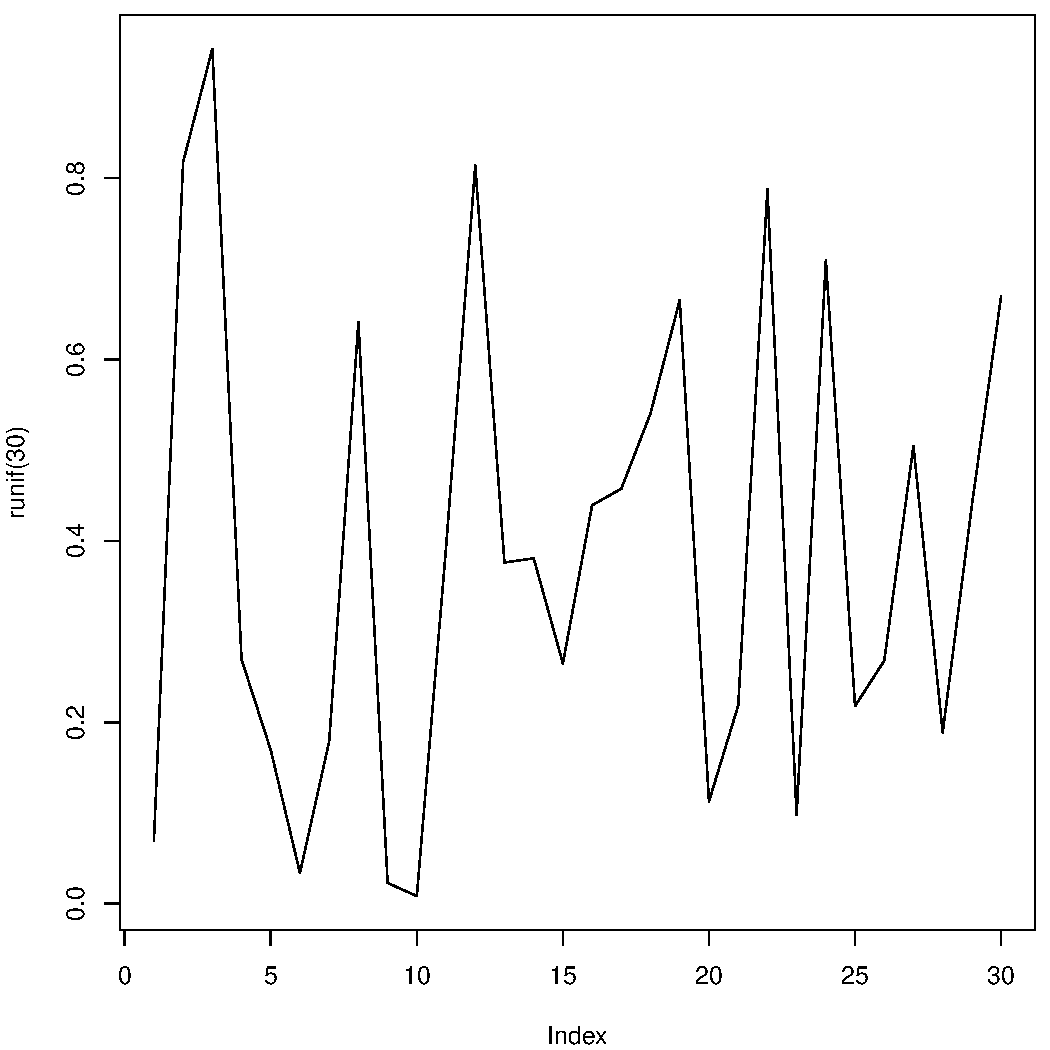
\includegraphics[width=\maxwidth]{figure/ch01_figunnamed-chunk-3-1} 

\end{knitrout}
  \caption{Test figure to illustrate figure options used by knitr.}
  \label{f02:1}
\end{figure}


% LaTeX file for Chapter 03


\chapter{Results}


% LaTeX file for Chapter 04


\chapter{Discussion and Outlook}



% LaTeX file for Chapter 05


\chapter{Conclusions}
\cleardoublepage
\phantomsection
\addtocontents{toc}{\protect \vspace*{10mm}}
\addcontentsline{toc}{chapter}{\bfseries Bibliography}


\bibliographystyle{mywiley} 
\bibliography{biblio}

\cleardoublepage

\end{document}



%%% Local Variables:
%%% ispell-local-dictionary: "en_US"
%%% End:
